%!TEX encoding = UTF-8 Unicode
%!TEX TS-program = XeLaTeX
%!TEX builder = latexmk
\documentclass[11pt,oneside,a4paper]{article}
\usepackage[parfill]{parskip}
  \setlength{\parindent}{0pt}%
  \setlength{\parskip}{6pt plus 2pt minus 4pt}%
  \setlength\abovedisplayskip{6pt plus 2pt minus 4pt}%
  \setlength\belowdisplayskip{6pt plus 2pt minus 4pt}%
  \setlength{\emergencystretch}{3em}%
  \frenchspacing

\lefthyphenmin=3
\righthyphenmin=3
\clubpenalty=10000
\widowpenalty=10000
\displaywidowpenalty=10000

\usepackage{fontspec,xfrac}
  \defaultfontfeatures{Mapping=tex-text}
  \setmainfont{sourceserifpro}[%
    Extension   = .otf,
    UprightFont = *-regular,
    ItalicFont  = *-italic,
    BoldFont    = *-semibold,
    BoldItalicFont = *-semibolditalic,
    Numbers={Lining}
  ]
\usepackage{polyglossia}
  \setdefaultlanguage{english}
  \setotherlanguage{sanskrit}
  \newfontfamily\sanskritfont{Source Serif Pro}

\usepackage{varwidth,xspace}
\newenvironment{shloka}[1]
  {\bigskip\center#1\varwidth{\linewidth}}
  {\endvarwidth\endcenter\bigskip}

\newcommand{\tl}[1]{\emph{#1}}

\addtocontents{toc}{\protect\thispagestyle{empty}} % Removes pagenumber appearing from TOC

% Colors, graphics and figures
\usepackage[usenames, dvipsnames]{xcolor}
\usepackage{latexcolors}
% \definecolor{darkpowderblue}{rgb}{0.0, 0.2, 0.6}
% \definecolor{cadmiumred}{rgb}{0.89, 0.0, 0.13}
\usepackage{graphicx}
  \setkeys{Gin}{width=\linewidth,totalheight=\textheight,keepaspectratio}
  \DeclareGraphicsExtensions{.png, .jpg, .pdf}

\usepackage{hyperref,url}
  \hypersetup{%
    breaklinks=true,%
    linktocpage,%
    colorlinks=true,%
    linkcolor=darkpowderblue,%
    urlcolor=darkpowderblue,%
    citecolor=darkpowderblue,%
    anchorcolor=darkpowderblue,%
    pdfdisplaydoctitle=true%
}
  \urlstyle{same}

% PDF meta-information
\AtBeginDocument{
  \hypersetup{%
    pdfcreator={XeLaTeX},%
    pdfproducer={LaTeX with hyperref and Xraum}%
  }
}
\title{\textbf{Śrī Svarṇākarṣaṇa Bhairava\\ mantra upāsanā}}
\author{\textsc{bhairava tantra}}
\date{\relax}
\hyphenation{svar-ṇā-kar-ṣa-ṇa ma-hā-prā-sā-da bhai-ra-va de-va-tā-yai ma-hā-bha-i-ra-vā-ya}

\begin{document}
\maketitle
\tableofcontents
\clearpage

\phantomsection
\addcontentsline{toc}{section}{Introduction}
\section*{Introduction}

The word Bhairava is made up of ``bha" + ``ra" + ``va". ``Bha" means
the sustenance of the universe and ``ra" means dissolution of the universe
and ``va" means manifestation of the universe. These are the prime qualities
of God (the Brahman) — creation, sustenance and dissolution. In the Bhairava
form of Śiva, His ultimate reality is coupled with the eternal awareness
of Śakti. The Svarṇākarṣaṇa Bhairava form is different from the forms of
Bhairava that we have discussed in ``Forms of Bhairava" and ``Pervasive
Bhairava". This Svarṇākarṣaṇa Bhairava form is considered as the Supreme
combination of Śiva and Śakti from where the Universe originates, sustains and
dissolves. The \tl{upāsanā} of Bhairava is considered indispensable for all
\tl{upāsakas} of Bhagavatī. Lord Bhairava is worshiped in various forms:

\begin{itemize}
  \item As the consort of Mahāvidyā Goddesses (Akṣōbhya Bhairava, Krodhabhairava, etc.)
  \item As the consort of the Mātṛkā group of deities (Asitāṅga Bhairava, Ruru Bhairava, etc.)
  \item As the son of Bhagavatī, Vaṭuka, who is indispensable to \tl{saparyā}, as is the Kumārī
  \item Various forms of Bhairavas who form the retinue of Bhagavatī invoked for protection such as Baḍabānala Bhairava, Ākāśabhairava, Unmatta Bhairava, etc.
  \item Special forms invoked for specific purposes by \tl{śākta}-s: Svarṇākarṣaṇa Bhairava for protection and prosperity, Sammōhana Bhairava (for enchantment), Svacchanda Bhairava (as Mahāguru in \tl{śrīkula krama} system), etc.
\end{itemize}

Śrī Svarṇākarṣaṇa Bhairava is an \tl{uttarāṃga} mantra to Mahāṣoḍaśī,
Mahāprāsāda and also Vanadurgā. His association with Śrī Vidyā and Māhātmya
are described in ``Sundarī Tantra''.

\begin{shloka}\itshape
  tripurāyāḥ pure ramye mūle kalpataroḥ śubhe \\
  sthitaḥ simhāsane tatra bhāti kaḥ puruṣaḥ paraḥ \\
  dāsībhūtā mahālakṣmīḥ purato yasya rājate \\
  tasya me devadevasya mahāmantraṃ vada prabho
\end{shloka}

Parvati questions thus: ``Lord! Who is the resplendent Puruśa seated on
a throne under the wish-fulfilling \tl{kalpavṛkśa} in the beautiful city of
Śrī Tripurasundarī (Śrīpuram)? Mahālakṣmī, the goddess of wealth, has stationed
herself in his service [1]. Please describe the great mantra of this deity.''

\begin{shloka}\itshape
  mahātripurasundaryāḥ pure bhogasamnvite \\
  mūle kalpatarormahāsane maṇivirājite \\
  svarṇākarṣaṇanāmā'sau bhāti śrībhairavaḥ svayam \\
  bhaktānāṃ tripurāmbāyāḥ dhanarāśipradāyakaḥ \\
  alakṣmīnāśanaḥ sākṣāt brahmaviṣṇuśivātmakaḥ
\end{shloka}

Śrī Dakṣinamurti replies thus: ``In the city of Śrī Mahātripurasundarī filled
with riches, seated on a gem-studded golden throne is the great Svarṇākarṣaṇa
Bhairava. He grants enormous wealth to the devotees of Śrī Tripurāmbika.
He destroys misfortune and his form constitutes of Brahmā-Viṣṇu-Rudra,
the trinity.''

\begin{shloka}\itshape
  brahmā nārāyaṇaḥ śambhurindrādyā lokapālakāḥ \\
  nityamenaṃ pūjayanti sampattyarthaṃ maheśvari \\
  sarvasampatprado nṝṇāṃ mahādāridryanāśakṛt
\end{shloka}

``The trinity, Indra and other deities worship him to obtain riches. He grants
prosperity to men and destroys poverty''.

\begin{shloka}\itshape
  purā pitāmaho devamenaṃ sampūjya bhairavam \\
  samprāpāṣṭaguṇaiśwaryam jagatkartṛtvamuttamam \\
  purā nārāyaṇaḥ sākṣāt swarṇākarṣaṇabhairavam \\
  śrīśatvamapa sampūjya dhanādhyakṣaṃ mahābalam \\
  aṇimādiguṇaiśvaryaṃ purā prāptaṃ mayā śive
\end{shloka}

``Even the trinity worshiped him to obtain the powers of creation, destruction
and sustenance''.

Mahādeva then goes on to describe the mantra [2] of The Lord and various
\tl{prayoga}-s to obtain unimagined riches [3]. As ``Sundarī Tantra'' [4] is
a Śrīkula---\tl{kādi krama ṭantra}, Svarṇākarṣaṇa Bhairava, described as
an \tl{aṇga} here, would pertain to \tl{kādi ṣoḍaśī}. ``Sundarī Tantra'' teaches
\tl{aṇga rāhitya} for \tl{pancadaśī}. Svarṇākarṣaṇa Bhairava is described as
one of the primary \tl{aṇga}-s of Śrīvidya in ``Dattātreya Samhitā''. He is
a part ofthe ``Raśmimala'', among the ``Chintāmaṇi Traya'' [5]. By
\tl{sampradaya}, Svarṇākarṣaṇa Bhairava is one of the sixteen \tl{aṇga}-s of
\tl{sādi vidyā saptadaśākṣarī}. The \tl{upāsanā} of Bhairava involves, along
with mantra, \tl{japa} and \tl{āvaraṇa pūjā}, recitation of \tl{mālā,
sahasranāma} [6], \tl{aṣṭottara, kavacha, stavarāja} and \tl{hṛdaya}.
The details of these however have to be received directly from one's Guru.

\textsc{notes}\footnote{Nirvāṇa Sundarī (\url{http://www.kamakotimandali.com/blog/})}:

[1] Mahālakṣmī is described as serving the Lord in various \tl{dhyāna śloka}-s
of this Bhairava. The ``Svarṇākarṣaṇa Aṣṭottara'' includes several names such
as: Mahālakṣmyarcitapadaḥ, Ramāpūjitapādābjaḥ, Vaikuṇṭhaśrīsamāśritaḥ, etc.
Mahālakṣmī and Madhumati are the two \tl{aṇgavidya}-s of Śrī Svarṇākarṣaṇa
Bhairava. ``Svarṇākarṣaṇa Bhairava Tantra'' (which most possibly is a part of
the bigger \tl{śaiva āgama}, ``Mahapanchākṣarī Tantra'', also housing other
smaller tantras such as ``Chidambara Tantra'') describes a story where
Mahālakṣmī lost her powers due to a curse by Śrī Durvasa Bhattaraka and
worshipped Bhairava at Avimukta kṣetra to regain her powers.

[2] The particular form of mantra described in ``Sundarī Tantra'' seems to be
the version used popularly by \tl{śrīvidyā upasaka}-s. For some reason, this
mantra is published in hundreds of corrupted forms in various manuals and these
corruptions can hardly be dismissed as \tl{pāṭhāntara}-s. There are two other
forms of mantra, one from an unknown source quoted in ``Āmnāya Kalpalatā'' (copied
as is in later works such as ``Amnaya Mantra Sangraha'', ``Saparya Paddhati'',
``Lalitarchana Chandrika'', etc.) and the other from ``Skanda Yāmala'' in
the ``Vanadurgā Mahāvidyā Prakaraṇa''. Though the mantra described in the context of
\tl{mahāvidyā} is different, most \tl{upāsaka}-s seem to use the first and
the popular version during recitation of \tl{panchaṣatī/saptaṣatī}. The only
\tl{sampradāya} which seems to use ``Skandayāmala'' as \tl{pramāṇa} is that of
Kalyanananda Bharati of Andhra Desha. They use a mixture of ``Vanadurgopaniṣad''
and ``Kalpa Kaustubha'' (of Rudrayamala) for the \tl{mūla pāṭha} of \tl{mahāvidyā
panchaśati} but utilize the \tl{aṇga-vidyā krama} of ``Skanda Yamala''. Of course,
everything said by Kalyanananda Bharati has to be consumed with a pinch of salt
and sometimes pepper too!

[3] The worship of Svarṇākarṣaṇa Bhairava is chiefly for prosperity and sudden
financial gains but that is not the sole benefit of this \tl{upāsanā}. He is
also an Apaduddharaṇa mūrti who destroys hindrances and protects the \tl{upāsaka}.
Svarṇākarṣaṇa Bhairava, famed to be stationed in Chidambaram in the service
of Śrī Chitasabhapati and Śrī Śivakamasundari, is described as \tl{bhairavo
viṣṇurūpakaḥ} in ``Chidambara Tantra''. He is thus identified as non-different
from Śrīmannarayana. He is further described as a combination of Samkarṣaṇa
and Bhairava \tl{svarupa}-s of Narayana and Mahādeva respectively. Due to
\tl{sattva prādhānya}, his mantra is considered ok to be given to women
(substituting the \tl{praṇava} with \tl{ramā bīja}) initiated into Śrīvidya
as women are prohibited from obtaining the mantra of Vaṭuka Bhairava
(``Hamsamāheshvara'', ``Rudrayāmala'', etc.). However, \tl{upāsana} of
Svarṇākarṣaṇa Bhairava mantra has to be undertaken only under the direct
guidance of Sadguru as the mantra activates \tl{kuhū nāḍi} and malfunctioning
of this \tl{nādī} can cause irreparable damage to a person. \tl{Kuhū} functions
towards ejaculation and its abuse can push the consciousness into netherworlds.

[4] ``Sundarī Tantra'' is described in the list of tantras speltout in ``Vārāhī
Tantra''. Another list, in yet another tantra, speaks of a ``Tripurasundarī
Tantra''. Some hold these two tantras to be the same. But Śrī Gopinath
Kaviraj-ji writes somewhere that the two are independent tantras. ``Sundarī
Tantra'' is available almost completely.

[5] The ``Chintāmaṇi Traya'' includes: Svarṇākarṣaṇa Bhairava, Ardhanārīśvara
Chintāmaṇi and Chintāmaṇi Ganapati.

[6] I have not personally seen the ``Sahasranāma of Śrī Svarṇākarṣaṇa Bhairava''
anywhere but have heard about the existence of one such \tl{sahasranāma} in
the possession of Ganapati Sacchidananda Swami of Mysore. Also, in the ``Uttara
Pīṭhikā'' of the ``Svarṇākarṣaṇa Hṛdaya'', there is a clear indication of
the existence of such a \tl{sahasranāma}. Śrī Svarṇākarṣaṇa Bhairava, Bhāgavan
Śrī Śuddha Dakśinamurti, Śrī Dattatreya, Bhāgavan Śrī Nṛsiṃha and Bhāgavan
Śrī Ucchiśta Maha Ganapati are said to be the five \tl{trimūrtyātmaka mūrti}-s
worshipped in the \tl{ūrdhāmnaya} of Kādi Krama Tantra. Even outside the realms
of the Śrīvidya Krama Tantra, they are described to be \tl{trimūrtyātmaka}.

\begin{shloka}\itshape
  sarvākāracidātmikāṃ sakaruṇāṃ siṃhāsanāṃ bhairavīm \\
  śikṣānugraharakṣaṇaikahṛdayāmāgneyamūrtiṃ śivām \\
  viśvatrāṇaparāyaṇāṃghrikamalāṃ kṣudrāśayakṣobhiṇīm \\
  devīṃ bhairava-vāmapakṣanilayāṃ durgām bhaje caṇḍikām
\end{shloka}

\begin{figure}[ht]
  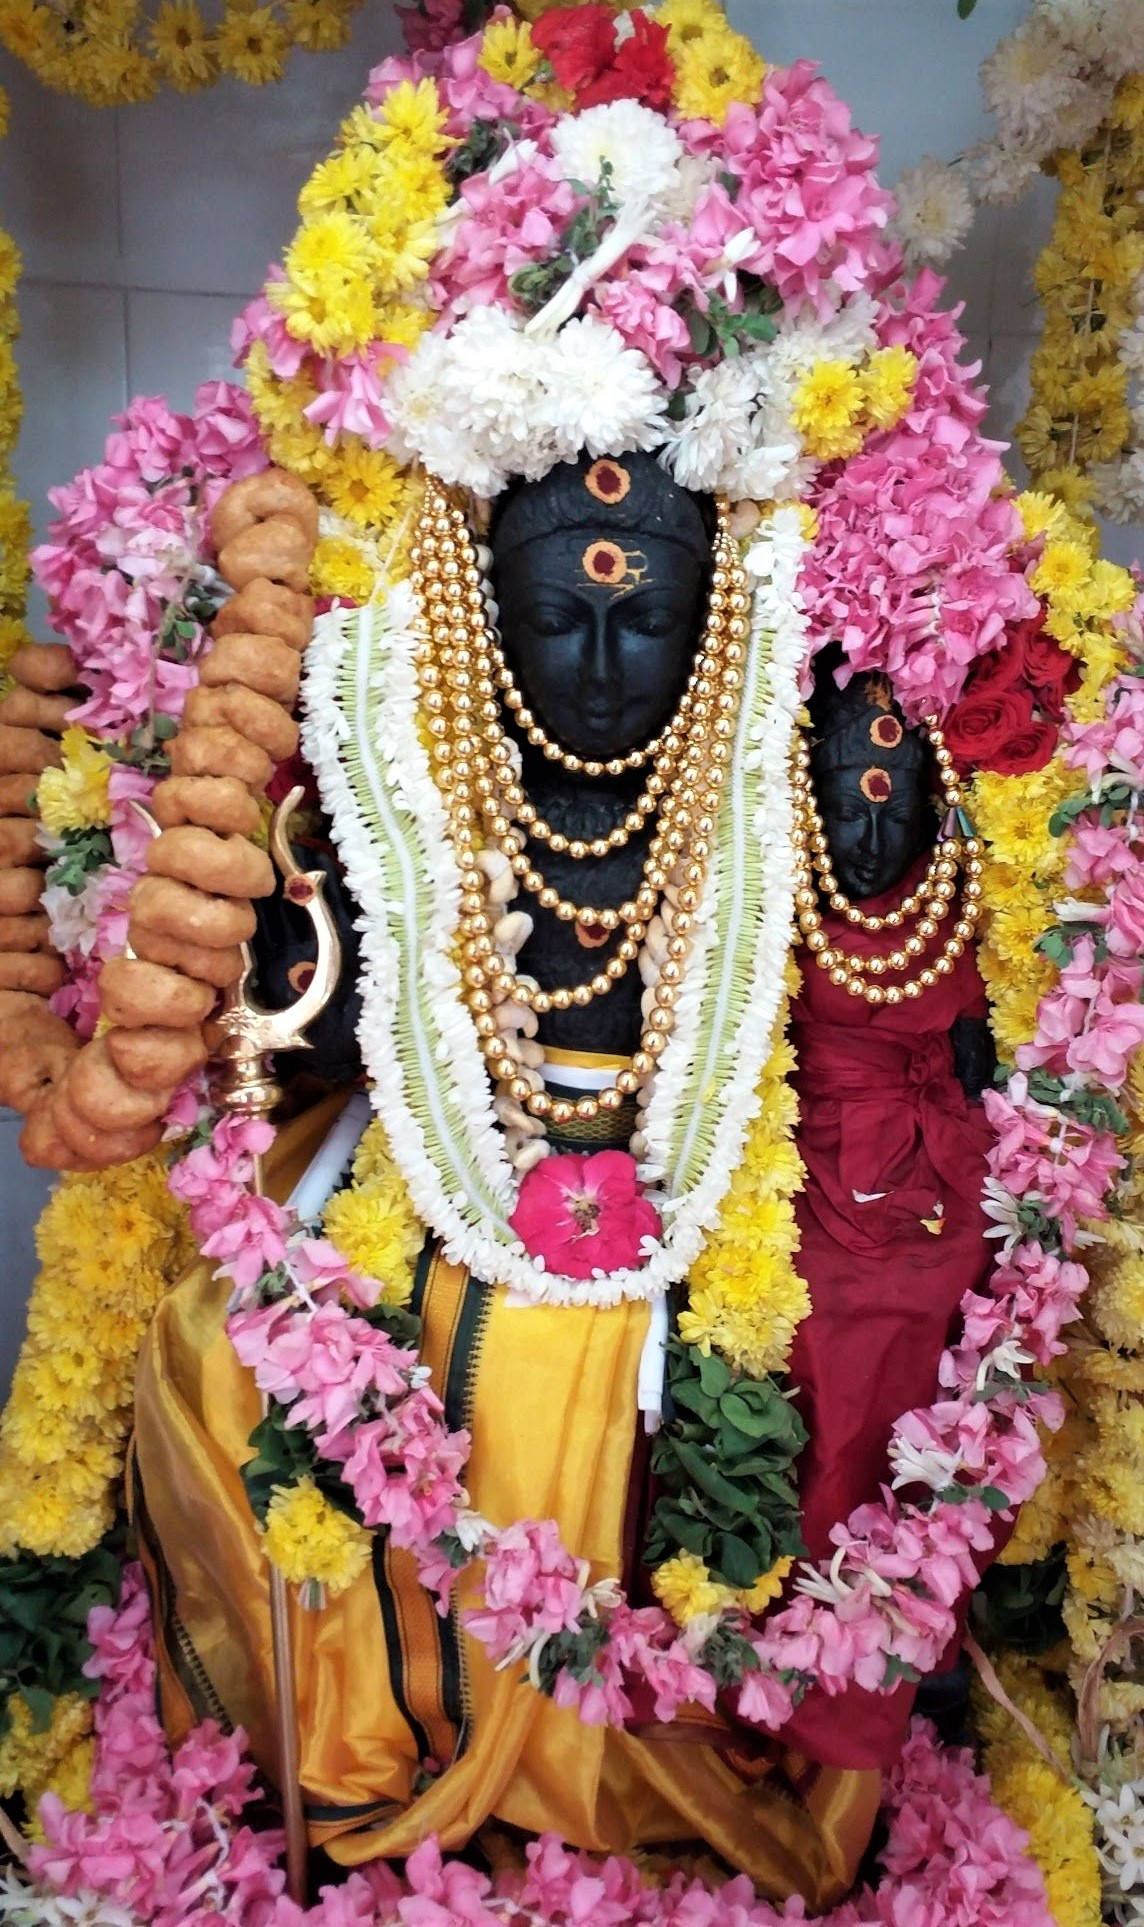
\includegraphics{svarnakarsana-bhairava.jpg}
\end{figure}
\clearpage

\section{Ṣaṭpañcāśatyakṣara mahāmantraḥ}
\subsection{Viniyogaḥ}

\begin{shloka}\itshape
  oṃ asyaśrī svarṇākarṣaṇa bhairava mantrasya \\
  śrī brahmā ṛṣiḥ paṅkti chandaḥ \\
  harihara brahmātmaka svarṇākarṣaṇa bhairavo devatā \\
  hrīṃ bījaṃ saḥ śaktiḥ oṃ kīlakaṃ \\
  mama dāridryanāśārthe svarṇākarṣaṇa bhairava prasāda siddhyarthaṃ \\
  svarṇa rāśi prāptyarthe svarṇākarṣaṇa bhairava mantra jape viniyogaḥ
\end{shloka}

The purpose of this \tl{sadhana} is to invoke Śrī Svarṇākarṣaṇa Bhairava and
perform His mantra \tl{japa} to obtain complete grace in all aspects,
specifically for removal of all types of poverty and acquisition of immense
wealth, as well as to gain peace of mind and contentment in life. The sage
(\tl{ṛṣiḥ}) is the divine seer Brahmā, the meter (\tl{chandas}) for the mantra
is \tl{paṅkti} and the deity is the intelligence giver Śrī Harihara Brahmātmaka
Svarṇākarṣaṇa Bhairava; the seed (\tl{bījaṃ}) is \tl{hrīṃ}, the power or
\tl{śakti} is \tl{saḥ}. The key (\tl{kīlakaṃ}) to unlock the mantra is oṃ.

\subsection{Ṛṣyādi nyāsa}

\tl{brahmā ṛṣaye namaḥ śirasi}\\
Open the right palm and touch the top of the forehead with the ring and thumb
fingers joined at the top.

\tl{paṅkti chandase namaḥ mukhe}\\
Now touch the lips of the mouth with the ring and thumb fingers joined at
the top.

\tl{brahmātmaka svarṇākarṣaṇa bhairava devatāyai namaḥ hṛdi}\\
Touch the heart area with the right palm.

\tl{hrīṃ bījāya namaḥ guhye}\\
Touch the genitalia area with the right ring finger and thumb joined together.

\tl{saḥ śaktaye namaḥ pādayoḥ}\\
Touch the feet area with the right ring finger and thumb joined together.

\tl{oṃ kīlakāya namaḥ nābhau}\\
Touch the navel area with the right ring finger and thumb joined together.

\tl{mama dāridryanāśārthe svarṇākarṣaṇa
bhairava prasāda svarṇa rāśi prāptyarthe svarṇākarṣaṇa bhairava mantra jape
viniyogāya namaḥ sarvāṅge}\\
Run both the palms all over the body.

\begin{shloka}\itshape
  iti ṛṣyādi nyāsaḥ
\end{shloka}

\subsection{Karanyāsaḥ}

\tl{aiṃ hrīṃ śrīṃ āparduddhāraṇāya aṅguṣṭhābhyāṃ namaḥ}\\
Use both the index fingers and run them on both the thumbs.

\tl{hrāṃ hrīṃ hrūṃ ajāmilabaddhāya tarjanībhyāṃ namaḥ}\\
Use both the thumbs and run them on both the index fingers.

\tl{oṃ lokeśvarāya madhyamābhyāṃ namaḥ}\\
Use both the thumbs on the middle fingers.

\tl{oṃ svarṇākarṣaṇa bhairavāya anāmikābhyāṃ namaḥ}\\
Use both the thumbs on the ring fingers.

\tl{mama dāridrya vidveṣaṇāya kaniṣṭhikābhyāṃ namaḥ}\\
Use both the thumbs on the little fingers.

\tl{mahā bhairavāya namaḥ karatalakarapṛṣṭhābhyāṃ namaḥ}\\
Open both the palms; run the opened palms of the right hand on the front and
back sides of the left palm and repeat the same for the other palm.

\begin{shloka}\itshape
  iti kara nyāsaḥ
\end{shloka}

\subsection{Ṣaḍaṅganyāsaḥ}

\tl{aiṃ hrīṃ śrīṃ āparduddhāraṇāya hṛdayāya namaḥ}\\
Open index, middle and ring fingers of the right hand and place them on
the heart area.

\tl{hrāṃ hrīṃ hrūṃ ajāmilabaddhāya śirase svāhā}\\
Open middle and ring fingers of the right hand and touch the top of
the forehead.

\tl{oṃ lokeśvarāya śikhāyai vaṣaṭ}\\
Open the right thumb and touch the back of the head. This is the point where
the tuft of hair is kept.

\tl{oṃ svarṇākarṣaṇa bhairavāya kavacāya huṃ}\\
Cross both the hands and run the fully opened palms from shoulders to finger
tips.

\tl{mama dāridrya vidveṣaṇāya netratrayāya vauṣaṭ}\\
Touch the eyes with the right index and ring fingers, with the middle finger
touching the \tl{ājña cakra}.

\tl{mahā bhairavāya namaḥ astrāya phaṭ}\\
Open up the left palm and strike it three times with index and middle fingers
of the right hand.

\tl{bhūr-bhuva-ssuvarom-iti digbandhaḥ}\\
May all the directions be sealed and may no thoughts or disturbances impact our
ability to recite the hymn.

\begin{shloka}\itshape
  iti ṣaḍaṅga nyāsaḥ
\end{shloka}

\subsection{Dhyānaṃ}

\begin{shloka}\itshape
  pītavarṇaṃ catur-bāhuṃ trinetraṃ pīta-vāsasam\\
  akṣyaṃ svarṇa-māṇikyaṃ taḍitapūrita pātrakam\\
  abhilaṣitaṃ mahā-śūlaṃ cāmaraṃ tomarodvaham\\
  svarṇābharaṇa-sampannaṃ muktāhāropaśobhitam (1)\\

  madonmattaṃ sukhāsīnaṃ bhaktānām ca vara pradam\\
  satataṃ cintaye devaṃ bhairavaṃ sarva-siddhidam\\
  pārijāta drumakāntārasthite maṇimaṇḍape\\
  siṃhāsanagataṃ dhyāyed bhairavaṃ svarṇadāyakam (2)\\

  gāṅgeyapātraṃ ḍamaruṃ triśūlaṃ varaṃ karaiḥ saṃdadhataṃ trinetraṃ\\
  devyāyutaṃ taptasvarṇavarṇa svarṇākṛtiṃ bhairavamāśrayāmi (3)\\
\end{shloka}

Salutations to Lord Svarṇākarṣaṇa Bhairava, who is yellowish gold in complexion
with four arms, three-eyed and adorned in golden garments. His eyes appear as
golden rubies and He is emanating brilliance resembling a lightning like bolt,
that engulfs the entire Creation. He readily grants all our cherished wishes
and desires. He is holding a \tl{trident} (to dispel all the triads), bearing
a whisk and a lance (to penetrate the \tl{cakra}-s) and is also adorned with all
types of precious and rare gems, gold and beautiful strings of pearls. He is
comfortably seated and intoxicated with bliss and is ready to fulfill all our
wishes. He is constantly reflecting upon and immersed in the welfare of the
Creation and is endowed with unlimited \tl{siddhi}-s. He is in the midst of
a forest full of the fragrant and mystical trees called \tl{pārijāta} and in
a hall of precious gems and crytals of unmatched beauty and glitter. He is to
be meditated as seated upon a royal lion faced throne and ready to bestow any
wish of His sincere devotees.

He is holding a bowl of water from the river Ganges, a musical drum, a trident
and displaying the wish granting \tl{varamudra}. He is three-eyed and is
worshipped by tens of thousands of \tl{deva}-s and other celestials. He is
radiant with a brilliant golden complexion and is the grantor of all types of
unimaginable prosperity. Salutations to Bhairava, the most merciful and generous
grantor of all types of abundance and prosperity!

\subsection{Pañcapūjā}

\tl{laṃ pṛthivyātmikāyai gandhaṁ samarpayāmi}\\
Hold the lower tip of the bottom phalange of the little fingers of both hands
with the upper tip of the thumbs, with the back of the hand facing us.

\tl{haṃ ākāśātmikāyai puṣpaiḥ pūjayāmi}\\
Hold the lower tip of the bottom phalange of the thumbs of both hands with
the upper tip/nails of the index fingers, with the back of the hand facing us.

\tl{yaṃ vāyvātmikāyai dhūpamāghrāpayāmi}\\
Hold the lower tip of the bottom phalange of the index fingers of both hands
with the upper tip of the thumbs, with the back of the hand facing us.

\tl{raṃ agnyātmikāyai dīpaṃ darśayāmi}\\
Hold the lower tip of the bottom phalange of the middle fingers of both hands
with the upper tip of the thumbs, with the back of the hand facing us.

\tl{vaṃ amṛtātmikāyai amṛtaṃ mahānaivedyaṃ nivedayāmi}\\
Hold the lower tip of the bottom phalange of the ring fingers of both hands with
the upper tip of the thumbs, with the back of the hand facing us.

\tl{saṃ sarvātmikāyai sarvopacāra pūjām samarpayāmi}\\
Hold the fingers of each palm in a folded manner with the tips of each fingers
of both hands touching each other and the thumbs facing the heart, in
a ``namaste'' position.

\subsection{Japamālā mantraṃ}

Recite the below mantra once, to pray to the \tl{japa māla} and invoke
the blessings for a fruitful \tl{japa}:

\begin{shloka}\itshape
  oṃ māṃ māle mahāmāye sarvamantra svarūpiṇi\\
  caturvarga stvayinyasta stasmānye siddhidā bhava
\end{shloka}

\subsection{Guru mantraḥ}

Recite the following guru mantra once, to seek the blessings of all gurus and
the Guru:

\begin{shloka}\itshape
  oṃ hrīṃ siddhaguro prasīda hrīṃ oṃ
\end{shloka}

\subsection{Ṣaṭpañcāśatyakṣara mantraḥ}

\begin{shloka}\itshape
  atha śrī svarṇākarṣaṇa bhairava ṣaṭpañcāśatyakṣara mantraḥ
\end{shloka}

Following is the 56-lettered Śrī Svarṇākarṣaṇa Bhairava mantra, that should be
recited at least 108 times (1 \tl{mālā}):

\begin{shloka}\itshape\bfseries
  oṃ aiṃ hrīṃ śrīṃ āpaduddhāraṇāya hrāṃ hrīṃ hrūṃ ajāmala-baddhāya lokeśvarāya
  svarṇākarṣaṇa bhairavāya mama dāridrya vidveṣaṇāya mahābhairavāya namaḥ
  śrīṃ hrīṃ aiṃ
\end{shloka}

The \tl{bīja} mantra \tl{oṃ} represents Śabda Brahman and is also called
the \tl{praṇava} mantra or the primordial sound, the manifested super-
consciousness in the form of sound and all syllables. All other sounds and waves
are said to have emanated from this mantra. The \tl{vāgbhāva bīja} mantra
\tl{aiṃ}, represents all knowledge, spiritual and material. The \tl{māyā bīja}
mantra \tl{hrīṃ} represents manifestation of everything as the power of Creation,
sustenance as the power of Preservation and transformation as the power of
Destruction. It is also related to concentration, focus, energy, drive,
self-esteem, high power and is the main \tl{śakti} mantra. The Lakṣmī \tl{bīja}
mantra \tl{śrīṃ}, represents abundance, wealth, well-being and prosperity,
as well as fructification of all efforts.

The word ‘\tl{āpaduddhāraṇāya}’ signifies — the one who rescues us from all
dangers and miserable conditions.

The \tl{bīja} mantra \tl{hrāṃ} pulls us away from karmic bonds and infuses
spirituality into our mind and intellect. The \tl{hrīṃ} \tl{bīja} mantra
represents the power of Destruction and applied to the individual self, it is
the destruction of our inner karmic bonds represented by \tl{antaḥkaraṇa} (mind,
ego and the intellect) that bind the consciousness to the physical, astral and
causal bodies. The form shifting \tl{kinnara bīja} mantra \tl{hrūṃ} brings
complete transformation in our spiritual outlook and leads us towards
self-realization. In this context Lord Bhairava is aided by the Divine Mother
Bhairavi, who wields the power of Destruction and transformation and is
the Destroyer of the Creation.

The word ‘\tl{ajāmala-baddhāya}’ is a combination of ‘\tl{aja}’ meaning —
leader, ‘\tl{amala}’ meaning — blemish-less and ‘\tl{baddhāya}’ meaning — bound.
He is a blemish-less leader and Lord and bound to the devotion of His devotees.
The word ‘\tl{lokeśvarāya}’ signifies — the Lord who rules over all the worlds
(and the Creation Itself). The word ‘\tl{svarṇākarṣaṇa}’ represents attraction
of all types of abundance including gold, precious gems, money, etc.
The word ‘\tl{bhairavāya}’ represents the Lord Bhairava, who is a terrific form
of Lord Śiva and is seen as a Protector. He is worshipped as a generous boon
giver by His devotees.

The word ‘\tl{mama}’ means myself/us. The word ‘\tl{dāridrya}’ means all types
of poverty, miseries and unfortunate conditions. The word ‘\tl{vidveṣaṇāya}’
signifies — the One who hates \tl{dāridrya}. The word ‘\tl{mahābhairavāya}’
represent Lord Śiva Himself as the chief Mahābhairava. The \tl{namaḥ} \tl{bīja}
mantra is for offering salutations to the deity and indicating our complete
surrender and request to the deity to take charge of our destiny.

The \tl{bīja} mantras \tl{śrīṃ}, \tl{hrīṃ} and \tl{aiṃ} are for encasing
the mantra for added protection and easier fruition. This process of reversing
the mantras at the end occurring earlier in the mantra, is called
\tl{sampuṭīkaraṇa}.

``Salutations to the Supreme Lord Svarṇākarṣaṇa Bhairava, the One who never fails
to come to the rescue of His devotees, relieve us of all karmas, infuse
uninhibited spirituality, material abundance and contentment in us and remove
all types of misery from our lives once and for all.''

\subsection{Gāyatrī mantraḥ}

Recite the Svarṇākarṣaṇa Bhairava \tl{gāyatrī} mantra 10 times or \sfrac{1}{10}
of main mantra \tl{japa}:

\begin{shloka}\itshape
  oṃ svarṇabhairavāya vidmahe\\
  svarṇākarṣaṇāya dhīmahi\\
  tanno bhairavaḥ pracodayāt
\end{shloka}

``May the golden complexioned Lord Svarṇākarṣaṇa Bhairava, the grantor of all
types of uninhibited abundance, kindle our intellect and illumine it!''

\subsection{Ṣaḍaṅganyāsaḥ}

\tl{aiṃ hrīṃ śrīṃ āparduddhāraṇāya hṛdayāya namaḥ}\\
Open index, middle and ring fingers of the right hand and place them on
the heart area.

\tl{hrāṃ hrīṃ hrūṃ ajāmilabaddhāya śirase svāhā}\\
Open middle and ring fingers of the right hand and touch the top of
the forehead.

\tl{oṃ lokeśvarāya śikhāyai vaṣaṭ}\\
Open the right thumb and touch the back of the head. This is the point where
the tuft of hair is kept.

\tl{oṃ svarṇākarṣaṇa bhairavāya kavacāya huṃ}\\
Cross both the hands and run the fully opened palms from shoulders to finger
tips.

\tl{mama dāridrya vidveṣaṇāya netratrayāya vauṣaṭ}\\
Touch the eyes with the right index and ring fingers, with the middle finger
touching the \tl{ājña cakra}.

\tl{mahā bhairavāya namaḥ astrāya phaṭ}\\
Open up the left palm and strike it three times with index and middle fingers
of the right hand.

\tl{bhūr-bhuva-ssuvarom-iti digbandhaḥ}\\
May all the directions be sealed and may no thoughts or disturbances impact our
ability to recite the hymn.

\begin{shloka}\itshape
  iti ṣaḍaṅga nyāsaḥ
\end{shloka}

\subsection{Dhyānaṃ}

\begin{shloka}\itshape
  pītavarṇaṃ catur-bāhuṃ trinetraṃ pīta-vāsasam\\
  akṣyaṃ svarṇa-māṇikyaṃ taḍitapūrita pātrakam\\
  abhilaṣitaṃ mahā-śūlaṃ cāmaraṃ tomarodvaham\\
  svarṇābharaṇa-sampannaṃ muktāhāropaśobhitam (1)\\

  madonmattaṃ sukhāsīnaṃ bhaktānām ca vara pradam\\
  satataṃ cintaye devaṃ bhairavaṃ sarva-siddhidam\\
  pārijāta drumakāntārasthite maṇimaṇḍape\\
  siṃhāsanagataṃ dhyāyed bhairavaṃ svarṇadāyakam (2)\\

  gāṅgeyapātraṃ ḍamaruṃ triśūlaṃ varaṃ karaiḥ saṃdadhataṃ trinetraṃ\\
  devyāyutaṃ taptasvarṇavarṇa svarṇākṛtiṃ bhairavamāśrayāmi (3)\\
\end{shloka}

\subsection{Pañcapūjā}

\tl{laṃ pṛthivyātmikāyai gandhaṁ samarpayāmi}\\
Hold the lower tip of the bottom phalange of the little fingers of both hands
with the upper tip of the thumbs, with the back of the hand facing us.

\tl{haṃ ākāśātmikāyai puṣpaiḥ pūjayāmi}\\
Hold the lower tip of the bottom phalange of the thumbs of both hands with
the upper tip/nails of the index fingers, with the back of the hand facing us.

\tl{yaṃ vāyvātmikāyai dhūpamāghrāpayāmi}\\
Hold the lower tip of the bottom phalange of the index fingers of both hands
with the upper tip of the thumbs, with the back of the hand facing us.

\tl{raṃ agnyātmikāyai dīpaṃ darśayāmi}\\
Hold the lower tip of the bottom phalange of the middle fingers of both hands
with the upper tip of the thumbs, with the back of the hand facing us.

\tl{vaṃ amṛtātmikāyai amṛtaṃ mahānaivedyaṃ nivedayāmi}\\
Hold the lower tip of the bottom phalange of the ring fingers of both hands with
the upper tip of the thumbs, with the back of the hand facing us.

\tl{saṃ sarvātmikāyai sarvopacāra pūjām samarpayāmi}\\
Hold the fingers of each palm in a folded manner with the tips of each fingers
of both hands touching each other and the thumbs facing the heart, in
a ``namaste'' position.

\subsection{Samarpaṇam}

Take water in \tl{uttaraṇi} (spoon) and by reciting the following \tl{śloka},
offer the water to the earth:

\begin{shloka}\itshape
  guhyātiguhyagoptrā tvaṁ gṛhāṇāsmat-kṛtaṁ japam\\
  siddhirbhavatu me deva tvatprasādānmayi sthirā
\end{shloka}

\subsection{Japānaṃtaraṃ mālāmantraṃ}

Recite the below \tl{śloka} and mantra, followed by placing the \tl{māla} upon
the top of the head and then place it back in the \tl{māla} bag and conceal it.
It should \textsc{\textbf{not}} be worn!

\begin{shloka}\itshape
  oṃ tvaṃ māle sarvadevānāṃ prītidā śubhadā bhava\\
  śubhaṃ kuruṣya me bhadre yaśo vīryaṃ ca dehime
\end{shloka}

\begin{shloka}\itshape
  oṃ hrīṃ siddhyai namaḥ
\end{shloka}

\subsection{Puraścaraṇa}

\tl{Japa}: 100,000, \tl{homa}: 10,000, \tl{tarpaṇa}: 1,000, \tl{mārjana} 100,
\tl{bhojana} 10.
\clearpage

\section{Aṣṭaṭpañcāśatyakṣara mahāmantraḥ}

\subsection{Viniyogaḥ}

\begin{shloka}\itshape
  oṃ asyaśrī svarṇākarṣaṇa bhairava mantrasya\\
  śrī brahmā ṛṣiḥ anuṣṭup chandaḥ\\
  śrī svarṇākarṣaṇa bhairava devatā\\
  hrīṃ bījaṃ klīṃ śaktiḥ saḥ kīlakaṃ\\
  mama sarva-kāma-siddhayarthe\\
  svarṇākarṣaṇa bhairava mantra jape viniyogaḥ
\end{shloka}

This mantra \tl{japa} is to invoke Śrī Svarṇākarṣaṇa Bhairava and perform His
mantra \tl{japa} to obtain His complete grace in all aspects, specifically for
removal of all types of poverty and acquisition of immense wealth, as well as
to gain peace of mind and contentment in life. With His blessings, one gains
complete happiness, abundance in wealth, etc. The sage (\tl{ṛṣiḥ}) is the divine
seer Brahmā, the meter (\tl{chandas}) for the mantra is \tl{anuṣṭup} and
the deity is the ultimate and unlimited wealth and prosperity giver Śrī
Svarṇākarṣaṇa Bhairava, the seed (\tl{bījaṃ}) is \tl{hrīṃ}, the power or
\tl{śakti} is \tl{klīṃ}. The key (\tl{kīlakaṃ}) to unlock the mantra
is \tl{saḥ}.

\subsection{Ṛṣyādi nyāsa}

\tl{brahmā ṛṣaye namaḥ śirasi}\\
Open the right palm and touch the top of the forehead with the ring and thumb
fingers joined at the top.

\tl{anuṣṭup chandase namaḥ mukhe}\\
Now touch the lips of the mouth with the ring and thumb fingers joined
at the top.

\tl{śrī svarṇākarṣaṇa bhairava devatāyai namaḥ hṛdi}\\
Touch the heart with the right palm.

\tl{hrīṃ bījāya namaḥ guhye}\\
Touch the genitalia with the right ring finger and thumb joined together.

\tl{klīṃ śaktaye namaḥ pādayoḥ}\\
Touch the feet with the right ring finger and thumb joined together.

\tl{saḥ kīlakāya namaḥ nābhau}\\
Touch the navel area with the right ring finger and thumb joined together.

\tl{mama sarva-kāma-siddhayarthe svarṇākarṣaṇa bhairava mantra jape viniyogāya
namaḥ sarvāṅge}\\
Run both the palms all over the body.

\begin{shloka}\itshape
  iti ṛṣyādi nyāsaḥ
\end{shloka}

\subsection{Karanyāsaḥ}

\tl{hrāṃ aṅguṣṭhābhyāṃ namaḥ}\\
Use both the index fingers and run them on both the thumbs.

\tl{hrīṃ tarjanībhyāṃ namaḥ}\\
Use both the thumbs and run them on both the index fingers.

\tl{hrūṃ madhyamābhyāṃ namaḥ}\\
Use both the thumbs on the middle fingers.

\tl{hraiṃ anāmikābhyāṃ namaḥ}\\
Use both the thumbs on the ring fingers.

\tl{hrauṃ kaniṣṭhikābhyāṃ namaḥ}\\
Use both the thumbs on the little fingers.

\tl{hraḥ karatalakarapṛṣṭhābhyāṃ namaḥ}\\
Open both the palms; run the opened palms of the right hand on the front and
back sides of the left palm and repeat the same for the other palm.

\begin{shloka}\itshape
  iti kara nyāsaḥ
\end{shloka}

\subsection{Ṣaḍaṅganyāsaḥ}

\tl{hrāṃ hṛdayāya namaḥ}\\
Open index, middle and ring fingers of the right hand and place them on
the heart.

\tl{hrīṃ śirase svāhā}\\
Open middle and ring fingers of the right hand and touch the top of the forehead.

\tl{hrūṃ śikhāyai vaṣaṭ}\\
Open the right thumb and touch the back of the head. This is the point where
the tuft of hair is kept.

\tl{hraiṃ kavacāya huṃ}\\
Cross both the hands and run the fully opened palms from shoulders to
finger tips.

\tl{hrauṃ netratrayāya vauṣaṭ}\\
Touch the eyes with the right index and ring fingers, with the middle finger
touching the \tl{ājña cakra}.

\tl{hraḥ astrāya phaṭ}\\
Open up the left palm and strike it three times with index and middle fingers
of the right hand.

\tl{bhūr-bhuva-ssuvarom-iti digbandhaḥ}\\
May all the directions be sealed and may no thoughts or disturbances impact our
ability to recite the hymn.

\begin{shloka}\itshape
  iti ṣaḍaṅga nyāsaḥ
\end{shloka}

\subsection{Dhyānaṃ}

\begin{shloka}\itshape
pītavarṇaṃ catur-bāhuṃ trinetraṃ pīta-vāsasam\\
akṣyaṃ svarṇa-māṇikyaṃ taḍitapūrita pātrakam\\
abhilaṣitaṃ mahā-śūlaṃ cāmaraṃ tomarodvaham\\
svarṇābharaṇa-sampannaṃ muktāhāropaśobhitam (1)\\

madonmattaṃ sukhāsīnaṃ bhaktānām ca vara pradam\\
satataṃ cintaye ddevaṃ bhairavaṃ sarva-siddhidam\\
pārijāta drumakāntārasthite maṇimaṇḍape\\
siṃhāsanagataṃ dhyāyed bhairavaṃ svarṇadāyakam (2)\\

gāṅgeyapātraṃ ḍamaruṃ triśūlaṃ varaṃ karaiḥ saṃdadhataṃ trinetraṃ\\
devyāyutaṃ taptasvarṇavarṇa svarṇākṛtiṃ bhairavamāśrayāmi (3)
\end{shloka}

Salutations to Lord Svarṇākarṣaṇa Bhairava, who is yellowish gold in complexion
with four arms, three-eyed and adorned in golden garments. His eyes appear as
golden rubies and He is emanating brilliance resembling a lightning like bolt,
that engulfs the entire Creation. He readily grants all our cherished wishes
and desires. He is holding a trident, bearing a whisk and a lance and is also
adorned with all types of precious and rare gems, gold and beautiful strings of
pearls. He is comfortably seated and intoxicated with bliss and is ready to
fulfill all our wishes. He is constantly reflecting upon and immersed in
the welfare of the Creation and is endowed with unlimited \tl{siddhi}-s. He is
in the midst of a forest full of the fragrant and mystical trees called
\tl{pārijāta} and in a hall of precious gems and crystals of unmatched beauty
and glitter. He is to be meditated as seated upon a royal lion faced throne and
ready to bestow any wish of His sincere devotees.

He is holding a golden bowl full of abundance, a musical drum, a trident and
displaying the wish granting \tl{vara mudra}. He is three-eyed and is worshipped
by tens of thousands of \tl{deva}-s and other celestials and is Himself
radiating with the glow equivalent to tens of thousands of celestials. He is
radiant with a brilliant golden complexion and is the grantor of all types of
unimaginable prosperity. Salutations to Bhairava, the most merciful and generous
grantor of all types of abundance and prosperity!

\subsection{Pañcapūjā}

\tl{laṃ pṛthivyātmikāyai gandhaṁ samarpayāmi}\\
Hold the lower tip of the bottom phalange of the little fingers of both hands
with the upper tip of the thumbs, with the back of the hand facing us.

\tl{haṃ ākāśātmikāyai puṣpaiḥ pūjayāmi}\\
Hold the lower tip of the bottom phalange of the thumbs of both hands with
the upper tip/nails of the index fingers, with the back of the hand facing us.

\tl{yaṃ vāyvātmikāyai dhūpamāghrāpayāmi}\\
Hold the lower tip of the bottom phalange of the index fingers of both hands
with the upper tip of the thumbs, with the back of the hand facing us.

\tl{raṃ agnyātmikāyai dīpaṁ darśayāmi}\\
Hold the lower tip of the bottom phalange of the middle fingers of both hands
with the upper tip of the thumbs, with the back of the hand facing us.

\tl{vaṃ amṛtātmikāyai amṛtaṁ mahānaivedyaṁ nivedayāmi}\\
Hold the lower tip of the bottom phalange of the ring fingers of both hands
with the upper tip of the thumbs, with the back of the hand facing us.

\tl{saṃ sarvātmikāyai sarvopacāra pūjām samarpayāmi}\\
Hold the fingers of each palm in a folded manner with the tips of each fingers
of both hands touching each other and the thumbs facing the heart in
a ``namaste'' position.

\subsection{Japamālā mantraṃ}

Recite the below mantra once to pray to the \tl{japa māla} and invoke
the blessings for a fruitful \tl{japa}:

\begin{shloka}\itshape
  oṃ māṃ māle mahāmāye sarvamantra svarūpiṇi\\
  caturvarga stvayinyasta stasmānye siddhidā bhava
\end{shloka}

\subsection{Guru mantraḥ}

Recite the following \tl{guru} mantra once, to seek the blessings of all
\tl{guru}-s and the Guru.

\begin{shloka}\itshape
  oṃ hrīṃ siddhaguro prasīda hrīṃ oṃ
\end{shloka}

\subsection{Aṣṭaṭpañcāśatyakṣara mantraḥ}

\begin{shloka}\itshape
  atha śrī svarṇākarṣaṇa bhairava aṣṭaṭpañcāśatyakṣara mantraḥ
\end{shloka}

Following is the 58-lettered Śrī Svarṇākarṣaṇa Bhairava mantra, that should be
recited at least 108 times (1 \tl{mālā}).

\begin{shloka}\itshape\bfseries
  oṃ aiṃ hrīṃ śrīṃ aiṃ śrīṃ āpaduddhāraṇāya hrāṃ hrīṃ hrūṃ ajāmala-baddhāya
  lokeśvarāya svarṇākarṣaṇa bhairavāya mama dāridrya vidveṣaṇāya
  mahābhairavāya namaḥ śrīṃ hrīṃ aiṃ
\end{shloka}

\subsection{Gāyatrī mantra}

Recite 10 times or \sfrac{1}{10} of main mantra \tl{japa}:

\begin{shloka}\itshape
  oṃ svarṇabhairavāya vidmahe\\
  svarṇākarṣaṇāya dhīmahi\\
  tanno bhairavaḥ pracodayāt
\end{shloka}

``May the golden complexioned Lord Svarṇākarṣaṇa Bhairava, the grantor of all
types of uninhibited abundance, kindle our intellect and illumine it!''

\subsection{Ṣaḍaṅganyāsaḥ}

\tl{hrāṃ hṛdayāya namaḥ}\\
Open index, middle and ring fingers of the right hand and place them on
the heart.

\tl{hrīṃ śirase svāhā}\\
Open middle and ring fingers of the right hand and touch the top of the forehead.

\tl{hrūṃ śikhāyai vaṣaṭ}\\
Open the right thumb and touch the back of the head. This is the point where
the tuft of hair is kept.

\tl{hraiṃ kavacāya huṃ}\\
Cross both the hands and run the fully opened palms from shoulders to
finger tips.

\tl{hrauṃ netratrayāya vauṣaṭ}\\
Touch the eyes with the right index and ring fingers, with the middle finger
touching the \tl{ājña cakra}.

\tl{hraḥ astrāya phaṭ}\\
Open up the left palm and strike it three times with index and middle fingers
of the right hand.

\tl{bhūr-bhuva-ssuvarom-iti digbandhaḥ}\\
May all the directions be sealed and may no thoughts or disturbances impact our
ability to recite the hymn.

\begin{shloka}\itshape
  iti ṣaḍaṅga nyāsaḥ
\end{shloka}

\subsection{Dhyānaṃ}

\begin{shloka}\itshape
pītavarṇaṃ catur-bāhuṃ trinetraṃ pīta-vāsasam\\
akṣyaṃ svarṇa-māṇikyaṃ taḍitapūrita pātrakam\\
abhilaṣitaṃ mahā-śūlaṃ cāmaraṃ tomarodvaham\\
svarṇābharaṇa-sampannaṃ muktāhāropaśobhitam (1)\\

madonmattaṃ sukhāsīnaṃ bhaktānām ca vara pradam\\
satataṃ cintaye ddevaṃ bhairavaṃ sarva-siddhidam\\
pārijāta drumakāntārasthite maṇimaṇḍape\\
siṃhāsanagataṃ dhyāyed bhairavaṃ svarṇadāyakam (2)\\

gāṅgeyapātraṃ ḍamaruṃ triśūlaṃ varaṃ karaiḥ saṃdadhataṃ trinetraṃ\\
devyāyutaṃ taptasvarṇavarṇa svarṇākṛtiṃ bhairavamāśrayāmi (3)
\end{shloka}

\subsection{Pañcapūjā}

\tl{laṃ pṛthivyātmikāyai gandhaṁ samarpayāmi}\\
Hold the lower tip of the bottom phalange of the little fingers of both hands
with the upper tip of the thumbs, with the back of the hand facing us.

\tl{haṃ ākāśātmikāyai puṣpaiḥ pūjayāmi}\\
Hold the lower tip of the bottom phalange of the thumbs of both hands with
the upper tip/nails of the index fingers, with the back of the hand facing us.

\tl{yaṃ vāyvātmikāyai dhūpamāghrāpayāmi}\\
Hold the lower tip of the bottom phalange of the index fingers of both hands
with the upper tip of the thumbs, with the back of the hand facing us.

\tl{raṃ agnyātmikāyai dīpaṁ darśayāmi}\\
Hold the lower tip of the bottom phalange of the middle fingers of both hands
with the upper tip of the thumbs, with the back of the hand facing us.

\tl{vaṃ amṛtātmikāyai amṛtaṁ mahānaivedyaṁ nivedayāmi}\\
Hold the lower tip of the bottom phalange of the ring fingers of both hands
with the upper tip of the thumbs, with the back of the hand facing us.

\tl{saṃ sarvātmikāyai sarvopacāra pūjām samarpayāmi}\\
Hold the fingers of each palm in a folded manner with the tips of each fingers
of both hands touching each other and the thumbs facing the heart in
a ``namaste'' position.

\subsection{Samarpaṇam}

Take water in \tl{uttaraṇi} (spoon) and by reciting the following \tl{śloka},
offer the water to the earth:

\begin{shloka}\itshape
  guhyātiguhyagoptrā tvaṁ gṛhāṇāsmat-kṛtaṁ japam\\
  siddhirbhavatu me deva tvatprasādānmayi sthirā
\end{shloka}

\subsection{Japānaṃtaraṃ mālāmantraṃ}

Recite the below \tl{śloka} and mantra, followed by placing the \tl{māla} upon
the top of the head and then place it back in the \tl{māla} bag and conceal it.
It should \textsc{\textbf{not}} be worn!

\begin{shloka}\itshape
  oṃ tvaṃ māle sarvadevānāṃ prītidā śubhadā bhava\\
  śubhaṃ kuruṣya me bhadre yaśo vīryaṃ ca dehime
\end{shloka}

\begin{shloka}\itshape
  oṃ hrīṃ siddhyai namaḥ
\end{shloka}

\subsection{Puraścaraṇa}

\tl{Japa}: 100,000, \tl{homa}: 10,000, \tl{tarpaṇa}: 1,000, \tl{mārjana} 100,
\tl{bhojana} 10.
\clearpage

\section{Svarṇākarṣaṇa Bhairava stotram}

\begin{shloka}\itshape
  śrī mārkaṇḍeya uvāca\\
  bhagavan pramathādhīśa śiva-tulya-parākrama\\
  pūrvam-ukta-stvayā mantraṃ bhairavasya mahātmanaḥ (1)
\end{shloka}

The divine seer Śrī Mārkaṇḍeya spoke thus: Salutations to the great lord
Bhairava, who is one and the same as Lord Śiva (Rudra), the Destroyer (of
ignorance), equal in all respects in His valor, courage, strength and power.
May we recite His mantras and meditate upon Lord Bhairava, who is none other
than the True Reality! May He confer all material and spiritual benefits upon
us and liberate us.

\begin{shloka}\itshape
  idānīṃ śrotum-icchāmi tasya stotram-anuttamaṃ\\
  tat kenoktaṃ purā stotraṃ paṭhanāt-tasya kiṃ phalam (2)
\end{shloka}

What is that \tl{stotra} that is claimed to be all powerful, fruitful for
fulfilling all wishes? What is it that is all accomplishing for those, who
recite it with full devotion and fervor to Lord Bhairava?

\begin{shloka}\itshape
  tat sarvaṃ śrotum-icchāmi, brūhi me nandikeśvara (3)
\end{shloka}

Oh faithful and kind Lord Nandikeśvara\footnote{Lord Nandi, the bull faced
attendant of Lord Śiva}, please narrate this \tl{stotram} in full and
enlighten me.

\begin{shloka}\itshape
  śrī nandikeśvara uvāca\\
  idaṃ brahman mahā-bhāga lokānām-upakāraka\\
  stotraṃ vaṭuka-nāthasya durlabhaṃ bhuvana-traye (4)
\end{shloka}

Lord Śrī Nandikeśvara spoke thus: This \tl{stotram} is of Brahman Himself,
manifested as Lord Vaṭuka-nātha\footnote{Vaṭuka Bhairava in the form of a boy},
extremely rare and difficult to find in all the three realms and dimensions.
It ushers in immense auspiciousness, opens up the doors to acquisition of
immense fortune and also confers immeasurable benefits to the entire world and
its populace.

Lord Vaṭuka Bhairava as Brahman manifests Himself as Viriñci Vaṭuka Bhairava,
who becomes the cause and mentor of the Creator — Lord Brahma, Mukunda Vaṭuka
Bhairava, who becomes the cause and mentor of the Preserver — Lord Viṣṇu and
lastly, Rudra Vaṭuka Bhairava, who becomes the cause and mentor of the Destroyer
— Lord Rudra. In another classification, Lord Vaṭuka Bhairava is equated with
Brahma, Lord Svarṇākarṣaṇa Bhairava with Lord Viṣṇu and Lord Kāla Bhairava with
Lord Rudra.

\begin{shloka}\itshape
  sarva-pāpa-praśamanaṃ sarva-sampatti-dāyakam\\
  dāridrya-śamanaṃ puṃsām-āpadā-bhaya-hārakam (5)
\end{shloka}

This \tl{stotram} removes all sins and bad karmas, bestows all types of wealth
and prosperity. Destroys all types of poverty, ignorance and allays all types
of fears and dangers, that one may perceive from any source. (All types of
enemies, black-magic and other types of negative influences will be totally
eradicated!).

\begin{shloka}\itshape
  aṣṭaiśvarya-pradaṃ nṛṇāṃ parājaya-vināśanam\\
  mahā-kānti-pradaṃ caiva soma-saundarya-dāyakam (6)
\end{shloka}

One will receive all the benefits, material and spiritual, including wealth,
knowledge, health, children, food, courage and means to undertake and accomplish
any task etc. There is absolutely nothing, that cannot be achieved by the grace
of Bhairava! There shall never be any fear of losing in any battle, competition
or in achieving any task of importance to us. He is brilliant in appearance and
emits light and grace across the entire Creation. Likewise, He is also as
beautiful and handsome, as the moon to look at.

\begin{shloka}\itshape
  mahā-kīrti-pradaṃ stotraṃ bhairavasya mahātmanaḥ\\
  na vaktavyaṃ nirācāre hi putrāya ca sarvathā (7)
\end{shloka}

One will obtain great recognition, fame and popularity by the grace of the great
Lord Bhairava. There is nothing more to speak or narrate, or even deliberate
upon, of any approved usages and rituals. This \tl{stotram} by Itself, has
the power to accomplish anything! One shall be blessed with illustrious children
and all types of comforts and pleasures, that one may seek!

\begin{shloka}\itshape
  śucaye guru-bhaktāya śucaye'pi tapasvine\\
  mahā-bhairava-bhaktāya sevite nirdhanāya ca (8)
\end{shloka}

One who has a clean heart and immense faith and devotion towards his guru,
one who is a very sincere and devoted meditation practitioner, one who has
absolute faith and unstinted devotion to Lord Bhairava, one who is willing to
serve without any expectations of garnering wealth.

\begin{shloka}\itshape
  nija-bhaktāya vaktavyam-anyathā śāpam-āpnuyāt\\
  stotram-etat bhairavasya brahma-viṣṇu-śivātmanaḥ (9)
\end{shloka}

One who is endowed with true devotion and spoken of highly by others and
everyone, may be blessed by the benefits that can be accrued by the recitation
of this \tl{stotram}. All other rogue elements should not be bestowed with this
\tl{stotram}, in order to prevent any accumulation of bad karma and curses.
May Lord Bhairava, who is none other than Brahman manifested as the Creator
Brahma, Preserver Viṣṇu and the Destroyer Śiva (Rudra), bless us immensely and
help fulfill all our cherished wishes and desires.

\begin{shloka}\itshape
  śṛṇuṣva brūhito brahman sarva-kāma-pradāyakam (10)
\end{shloka}

Hear now very attentively, Oh pious and learned one, the stotram of Brahman
Himself, manifested as Śrī Svarṇākarṣaṇa Bhairava, the grantor of all wishes
and desires, the fulfiller of all tasks!

\subsection{Viniyogaḥ}

\begin{shloka}\itshape
  oṃ asya śrī-svarṇākarṣaṇa-bhairava-stotrasya\\
  brahmā ṛṣiḥ anuṣṭup chandaḥ\\
  śrī-svarṇākarṣaṇa-bhairava-devatā\\
  hrīṃ bījaṃ klīṃ śakti saḥ kīlakam\\
  mama-sarva-kāma-siddhayarthe pāṭhe viniyogaḥ (11)
\end{shloka}

This mantra \tl{japa} is to invoke Śrī Svarṇākarṣaṇa Bhairava and perform His
\tl{stotra japa} to obtain His complete grace in all aspects, specifically for
all types of wish fulfillment and accomplishment of all tasks. The sage
(\tl{ṛṣiḥ}) is the divine seer and Creator Brahma, the meter (\tl{chandas}) for
the mantra is Anuṣṭup and the deity is the ultimate and unlimited wealth giver —
Śrī Svarṇākarṣaṇa Bhairava, the seed (\tl{bījaṃ}) is \tl{hrīṃ}, the power or
\tl{śakti} is \tl{klīṃ}. The key (\tl{kīlakaṃ}) to unlock the mantra is \tl{saḥ}.

\subsection{Ṛṣyādi nyāsa}

\tl{brahmā ṛṣaye namaḥ śirasi}\\
Open the right palm and touch the top of the forehead with the ring and thumb
fingers joined at the top.

\tl{anuṣṭup chandase namaḥ mukhe}\\
Now touch the lips of the mouth with the ring and thumb fingers joined at
the top.

\tl{śrī svarṇākarṣaṇa bhairava devatāyai namaḥ hṛdi}\\
Touch the heart area with the right palm.

\tl{hrīṃ bījāya namaḥ guhye}\\
Touch the genitalia area with the right ring finger and thumb joined together.

\tl{klīṃ śaktaye namaḥ pādayoḥ}\\
Touch the feet with the right ring finger and thumb joined together.

\tl{saḥ kīlakāya namaḥ nābhau}\\
Touch the navel with the right ring finger and thumb joined together.

\tl{mama-sarva-kāma-siddhayarthe pāṭhe viniyogāya namaḥ sarvāṅge}\\
Run both the palms all over the body.

\begin{shloka}\itshape
  iti ṛṣyādi nyāsaḥ
\end{shloka}

\subsection{Karanyāsaḥ}

\tl{hrāṃ aṅguṣṭhābhyāṃ namaḥ}\\
Use both the index fingers and run them on both the thumbs.

\tl{hrīṃ tarjanībhyāṃ namaḥ}\\
Use both the thumbs and run them on both the index fingers.

\tl{hrūṃ madhyamābhyāṃ namaḥ}\\
Use both the thumbs on the middle fingers.

\tl{hraiṃ anāmikābhyāṃ namaḥ}\\
Use both the thumbs on the ring fingers.

\tl{hrauṃ kaniṣṭhikābhyāṃ namaḥ}\\
Use both the thumbs on the little fingers.

\tl{hraḥ karatalakarapṛṣṭhābhyāṃ namaḥ}\\
Open both the palms; run the opened palms of the right hand on the front and
back sides of the left palm and repeat the same for the other palm.

\begin{shloka}\itshape
  iti kara nyāsaḥ
\end{shloka}

\subsection{Ṣaḍaṅganyāsaḥ}

\tl{hrāṃ hṛdayāya namaḥ}\\
Open index, middle and ring fingers of the right hand and place them on
the heart \tl{cakra}.

\tl{hrīṃ śirase svāhā}\\
Open middle and ring fingers of the right hand and touch the top of
the forehead.

\tl{hrūṃ śikhāyai vaṣaṭ}\\
Open the right thumb and touch the back of the head. This is the point where
the tuft of hair is kept.

\tl{hraiṃ kavacāya huṃ}\\
Cross both the hands and run the fully opened palms from shoulders to
finger tips.

\tl{hrauṃ netratrayāya vauṣaṭ}\\
Touch the eyes with the right index and ring fingers, with the middle finger
touching the \tl{ājña cakra}.

\tl{hraḥ astrāya phaṭ}\\
Open up the left palm and strike it three times with index and middle fingers
of the right hand.

\tl{bhūr-bhuva-ssuvarom-iti digbandhaḥ}\\
May all the directions be sealed and may no thoughts or disturbances impact our
ability to recite the hymn.

\begin{shloka}\itshape
  iti ṣaḍaṅga nyāsaḥ
\end{shloka}

\subsection{Dhyānaḥ}

\begin{shloka}\itshape
  mandāra-druma-mūla-bhāji vijite ratnāsane saṃsthite\\
  divyaṃ cāruṇa-cañcukādhara-rucā devyā kṛtāliṅganaḥ (12)
\end{shloka}

Salutations to the Divine Lord, who resides in the midst of a \tl{mandāra}
forest, unrivalled, powerful and radiant. Seated on a bejeweled throne, shining
forth with red radiant beams of light, looking extremely handsome with
a chiseled face and is lovingly hugged by His consort Bhairavi.

\begin{shloka}\itshape
  bhaktebhyaḥ kara-ratna-pātra-bharitaṃ svarṇa dadhāno bhṛśam\\
  svarṇākarṣaṇa-bhairavo bhavatu me svargāpavarga-pradaḥ (13)
\end{shloka}

Behold the One who has many devotees! The Divine Father is holding a vessel full
of rare gems and treasures, gold and all types of riches. A vessel that can
never be emptied and He showers His grace again and again upon His devotees and
loads them with extreme prosperity and finally granting them liberation. Let us
meditate upon the most magnanimous Lord Svarṇākarṣaṇa Bhairava!

\begin{shloka}\itshape
  pārijāta druma kāntāre sthite māṇikya-maṇḍape\\
  siṃhāsana gataṃ vande bhairavaṃ svarṇa-dāyakaṃ (14)
\end{shloka}

He is in the midst of a forest full of the fragrant and mystical trees called
\tl{pārijāta} and in a hall of precious gems and crystals of unmatched beauty
and glitter. He is to be meditated as, seated upon a royal lion faced throne
and ready to bestow all types of riches as well as any wish of His sincere
devotees.

\begin{shloka}\itshape
  gāṅgeya pātraṃ ḍamarūṃ triśūlaṃ varaṃ karaḥ sandadhataṃ trinetraṃ\\
  devyāyutaṃ tapta-svarṇa-varṇa svarṇākarṣaṇa-bhairavam-āśrayāmi (15)
\end{shloka}

He is holding a golden vessel (\tl{kalaśa}) full of precious stones, gold and
all types of wealth\footnote{Alternately, \tl{gāṅgeya pātraṃ} can also mean
a vessel holding the water from the sacred Ganges river, but it is not
applicable in this context}, a musical drum\footnote{Emanates all mystical
vibrations, syllable \tl{mātṛka}-s}, a trident and displaying the wish granting
\tl{vara mudra}. He is three-eyed and is worshipped by tens of thousands of
\tl{devas} and other celestials. He is radiant with a brilliant golden
complexion and is the grantor of all types of unimaginable prosperity.
Salutations to Bhairava, the most merciful and generous grantor of all types
of abundance and prosperity!

\subsection{Mantraḥ}

\begin{shloka}\itshape\bfseries
  oṃ aiṃ hrīṃ śrīṃ aiṃ śrīṃ āpaduddhāraṇāya hrāṃ hrīṃ hrūṃ ajāmala-baddhāya
  lokeśvarāya svarṇākarṣaṇa bhairavāya mama dāridrya vidveṣaṇāya mahābhairavāya
  namaḥ śrīṃ hrīṃ aiṃ (16)
\end{shloka}

The \tl{bīja} mantra \tl{oṃ} represents Śabda Brahman and is also called
the \tl{praṇava} mantra or the primordial sound, the manifested
super-consciousness in the form of sound and all syllables. All other sounds
and waves are said to have emanated from this mantra. The \tl{vāgbhāva}
\tl{bīja} mantra \tl{aiṃ} represents all knowledge, spiritual and material.
The \tl{māyā} \tl{bīja} mantra \tl{hrīṃ} represents manifestation of everything
as the power of Creation, sustenance as the power of Preservation and
transformation as the power of Destruction. It is also related to concentration,
focus, energy, drive, self-esteem, high power and is the main \tl{śakti} mantra.
The Lakṣmī \tl{bīja} mantra \tl{śrīṃ} represents abundance, wealth, well-being
and prosperity, as well as fructification of all efforts.

The second \tl{vāgbhāva} \tl{bīja} mantra \tl{aiṃ} re-iterates the need to
obtain all the knowledge we need to succeed in all our tasks and become
accomplished. The second Lakṣmī \tl{bīja} mantra \tl{śrīṃ} indicates the desire
for fruition of all our efforts.

The word ‘\tl{āpaduddhāraṇāya}’ signifies the one who rescues us from all
dangers and miserable conditions.

The \tl{bīja} mantra \tl{hrāṃ} pulls us away from karmic bonds and infuses
spirituality into our mind and intellect. The \tl{hrīṃ} \tl{bīja} mantra
represents the power of Destruction and applied to the individual self, it is
the destruction of our inner karmic bonds represented by \tl{antaḥkaraṇa}
(mind, ego and the intellect) that bind the consciousness to the physical,
astral and causal bodies.

The form shifting \tl{kinnara bīja} mantra \tl{hrūṃ}, brings complete
transformation in our spiritual outlook and leads us towards self-realization.
In this context Lord Bhairava is aided by the Divine Mother Bhairavi, who wields
the power of Destruction and transformation and is the Destroyer of
the Creation.

The word ‘\tl{ajāmala-baddhāya}’ is a combination of ‘\tl{aja}’ meaning — leader,
‘\tl{amala}’ meaning — blemish-less and ‘\tl{baddhāya}’ meaning — bound. He is
a blemish-less leader and Lord and bound to the devotion of His devotees.
The word ‘\tl{lokeśvarāya}’ signifies — the Lord who rules over all the worlds.

The word ‘\tl{svarṇākarṣaṇa}’ represents attraction of all types of abundance
including gold, precious gems, money etc. The word ‘\tl{bhairavāya}’ represents
the Lord Bhairava, who is a terrific form of Lord Śiva and is seen as
a Protector. He is worshipped as a generous boon giver by His devotees.

The word ‘\tl{mama}’ means myself/us. The word ‘\tl{dāridrya}’ means all types
of poverty, miseries and unfortunate conditions. The word ‘\tl{vidveṣaṇāya}’
signifies — the One who hates \tl{dāridrya}. The word ‘\tl{mahābhairavāya}’
represent Lord Śiva Himself as the chief Mahābhairava.

The \tl{namaḥ bīja} mantra is for offering salutations to the deity and
indicating our complete surrender and request to the deity to take charge of
our destiny. The \tl{bīja} mantras \tl{śrīṃ}, \tl{hrīṃ} and \tl{aiṃ} are for
encasing the mantra for added protection and easier fruition. This process of
reversing the mantras at the end occurring earlier in the mantra, is called
\tl{sampuṭīkaraṇa}.

``Salutations to the Supreme Lord Svarṇākarṣaṇa Bhairava, the One who never
fails to come to the rescue of His devotees, relieve us of all karmas, infuse
uninhibited spirituality, material abundance and contentment in us and remove
all types of misery from our lives once and for all''.

\subsection{Stotra-pāṭha}

\begin{shloka}\itshape
  sarvajñāya namas-tubhyaṃ namaste divya-cakṣuṣe\\
  ajitāya namas-tubhyaṃ jita-mitrāya te namaḥ (24)
\end{shloka}

Salutations to the One who is the repository of all knowledge and holds
the power of Divine foresight and is the cause of all happenings. He can never
be conquered or subdued by any means and is also an ally of those who are
subdued and seeking His protection. Salutations to the great Lord Bhairava!

\begin{shloka}\itshape
  namaste rudra-rūpāya mahāvīrāya te namaḥ\\
  namo'sttv-ananta-vīryāya mahāghorāya te namaḥ (25)
\end{shloka}

Salutations to the One who is in the form of Lord Rudra, the Destroyer and
possessor of immense strength, potential and humungous power manifested in
the Creation. Salutations to the One who is verily the source of infinite power,
will and courage. Salutations to the One who is also the most terrific and
benevolent, as need be.

\begin{shloka}\itshape
  namaste ghora-ghorāya viśva-ghorāya te namaḥ\\
  namaḥ ugrāya śāntāya bhaktānāṃ śānti-dāyine (26)
\end{shloka}

Salutations to the One who is the most benevolent and terrific and is also
the Destroyer of the entire Creation, at the time of its dissolution.
Salutations to the most aggressive and war like, as well as the most composed
and peaceful and the greatest beneficent to all His devotees, in bestowing
everlasting happiness, comfort, joy and peace.

\begin{shloka}\itshape
  gurave sarva-lokānāṃ namaḥ praṇava-rūpiṇe\\
  namaste vāgbhav-ākhyāya dīrgha-kāmāya te namaḥ (27)
\end{shloka}

Salutations to the Divine Father, who is the teacher and guru of the entire
Creation and who is present in the form of the praṇava mantra \tl{oṃ}.
Salutations to the great lord, who is omnipresent in the meaning of all
the letters of the alphabet, including the alphabet and all the words and sound
frequencies. Salutations to Him, who is the Creator and the doer of all major
tasks and accomplishments and everything that is manifested in the Creation!

\begin{shloka}\itshape
  namaste kāma-rājāya yoṣita-kāmāya te namaḥ\\
  dīrgha-māyā-svarūpāya mahā-māyāya te namaḥ (28)
\end{shloka}

Salutations to the One who is the embodiment of all love, adoration, affection,
lust and all types of emotions. Salutations to the One who showers His affection
and grace upon all women and empowers them to accomplish any task! Salutations
to the One, who has unleashed the great cosmic illusion, called the Mahāmāya
and is omnipresent within it and embodies it as well.

\begin{shloka}\itshape
  sṛṣṭi-māyā-svarūpāya nisarga-samayāya te\\
  sura-loka-supūjyāya āpad-uddhāraṇāya ca (29)
\end{shloka}

Salutations to the One, who is the embodiment of the cosmic illusion, that
engulfs the entire Creation and generates a false sense of reality, that
the unenlightened beings perceive. Salutations to the One who creates
the perception of time and dispenses with it as desired. Salutations to the One
who is prayed to at all times by the celestials and the One who comes to their,
as well as to our rescue, during all crises and when most needed. Salutations
to the One who never refuses to come to the rescue of His devotees and is always
there, when called upon!

\begin{shloka}\itshape
  namo namo bhairavāya mahā-dāridrya-nāśine\\
  unmūlane karmaṭhāya alakṣmyāḥ sarvadā namaḥ (30)
\end{shloka}

Salutations to the Divine Bhairava, who destroys and eliminates even the worst
cases of poverty. He skillfully uproots the poverty causing elements and
provides the much needed succor, to all His devotees seeking His grace.

\begin{shloka}\itshape
  namo ajāmala-baddhāya namo lokeśvarāya te\\
  svarṇākarṣaṇa-śīlāya bhairavāya namo namaḥ (31)
\end{shloka}

Salutations to the blemish-less Lord bound to the sincere devotion of His
devotees and is the ruler of the entire Creation! Salutations to Bhairava, who
showers all types of riches and prosperity as is His natural dispensation,
to enrich His devotees and fulfill all their wants and protect them from
all harm.

\begin{shloka}\itshape
  mama dāridrya vidveṣaṇāya lakṣyāya te namaḥ\\
  namo loka-trayeśāya svānandaṃ nihitāya te (32)
\end{shloka}

Salutations to the Lord, who detests and removes all of our unfortunate
dispensations, financial crises, loans, debts and lack of prosperity. It becomes
an objective to the Divine Lord, to come to the rescue of His devotees and
ensure their well-being. Salutations to the Lord of all the three realms, who is
self-sufficient and ever content in His disposition.

\begin{shloka}\itshape
  namaḥ śrī-bīja-rūpāya sarva-kāma-pradāyine\\
  namo mahā-bhairavāya śrī-bhairava namo namaḥ (33)
\end{shloka}

Salutations to the Divine Lord who is in the form of the \tl{śrī bīja śrīṃ},
indicating prosperity, abundance and fertility. He is the fulfiller of all
desires and wishes of His sincere devotees. Salutations to the One who is none
other than Brahman, manifested as Lord Mahā Bhairava and as the Preserver and
Sustainer Lord Śrī Bhairava.

\begin{shloka}\itshape
  dhan-ādhyakṣa namas-tubhyaṃ śaraṇyāya namo namaḥ\\
  namaḥ prasanna ādi-devāya te namaḥ (34)
\end{shloka}

Salutations to the Divine Lord, who is the Lord of all wealth and is
the Protector and savior of the entire Creation. Salutations to the Divine Lord
manifested as the Creator Ādi Deva.

\begin{shloka}\itshape
  namaste mantra-rūpāya namaste mantra-rūpiṇe\\
  namaste svarṇa-rūpāya suvarṇāya namo namaḥ (35)
\end{shloka}

Salutations to the Divine Lord, who is in the form of the mantra Itself and is
also its power (\tl{śakti}). Salutations to the Divine Lord, who is golden
yellow in complexion and has a brilliant glow and golden hue.

\begin{shloka}\itshape
  namaḥ suvarṇa-varṇāya mahā-puṇyāya te namaḥ\\
  namaḥ śuddhāya buddhāya namaḥ saṃsāra-tāriṇe (36)
\end{shloka}

Salutations to the one, who is golden yellow in complexion and is most
auspicious, sinless and is purity personified. Salutations to the One who is
cleansed of all karmas, belongings and obsessions and is the superintelligence
Itself. Salutations to Him, who is our protector and sustainer and will carry us
through the journey of life and takes care of all our needs and that of
our family.

\begin{shloka}\itshape
  namo devāya guhyāya pracalāya namo namaḥ\\
  namaste bāla-rūpāya pareśāṃ balanāśine (37)
\end{shloka}

Salutations to the Divine Lord, who is all powerful, subtle, static and mobile
and is omnipresent everywhere. Salutations to the One who is in the form of
a lad as Vaṭuka Bhairava, representing the Creation Itself (Lord Brahma) and is
the Supreme Reality — Brahman with imperishable power and sustenance. As Lord
Rudra, He is also the Supreme power that destroys the entire Creation during
the time of dissolution.

\begin{shloka}\itshape
  namaste svarṇa saṃsthāya namo bhūtala-vāsine\\
  namaḥ pātāla-vāsāya anādhārāya te namaḥ (38)
\end{shloka}

Salutations to the One who is equated to the precious gold deposits on
the Earth’s surface and One who is omnipresent on the Earth’s surface to assist
His sincere devotees. Salutations to the One who is also present in the Earth’s
crust and the netherworlds and dimensions to assist His sincere devotees.
Salutations to the One, who needs no support or assistance to act upon or to
sustain Himself!

\begin{shloka}\itshape
  namo namaste śāntāya anantāya namo namaḥ\\
  dvi-bhujāya namas-tubhyaṃ bhuja-traya-suśobhine (39)
\end{shloka}

Salutations to the One who is calm and composed and ushers in peace to all
the realms. Salutations to the One who is eternal, infinite and omnipresent.
Salutations to the One who has two arms and sometimes dazzles the realms with
three arms (manifesting the triads).

\begin{shloka}\itshape
  namo'namādi siddhāya svarṇa-hastāya te namaḥ\\
  pūrṇa-candra-pratīkāśa vadan-āmbhoja-śobhine (40)
\end{shloka}

Salutations to the One who is the Supreme Self and bows to none and is the first
Siddha, the realized One! Salutations to the One whose hands are of gold.
Salutations to the One who is as magnetic in appearance as a full moon in its
golden disc form. Salutations to the One whose face dazzles and entices like
a blossomed lotus.

\begin{shloka}\itshape
  namaste'stu-svarūpāya svarṇ-ālaṅkāra-śobhine\\
  namaḥ svarṇ-ākarṣaṇāya svarṇ-ābhāya namo namaḥ (41)
\end{shloka}

Salutations to the One who is in His own mysterious form and can manifest
anywhere and in anything, throughout the Creation. Salutations to the One who is
bedecked in golden ornaments and dazzling with brilliance of golden hue.
Salutations to the One whose worship attracts wealth, abundance and immense
prosperity. Salutations to the one who looks very enticing and pleasing in
a golden appearance.

\begin{shloka}\itshape
  namaste svarṇa-kaṇṭhāya svarṇābhāmbara-dhāriṇe\\
  svarṇa-siṃhāsana-sthāya svarṇa-pādāya te namaḥ (42)
\end{shloka}

Salutations to the One who is golden throated and is adorned in golden garments.
Salutations to the One, who is seated on a golden lion faced throne and has
golden feet!

\begin{shloka}\itshape
  namaḥ svarṇabha-pādāya svarṇa-kāñcī-suśobhine\\
  namaste svarṇa-jaṅghāya bhakta-kāmad-uddhātmane (43)
\end{shloka}

Salutations to the One, who has golden feet and dazzles with golden girdles
around His waist and hips. Salutations to the One who has golden shanks (legs).
Salutations to the One, who extricates and fulfills all the inner desires of
His devotees.

\begin{shloka}\itshape
  namaste svarṇa-bhaktāya kalpavṛkṣa-svarūpiṇe\\
  cintāmaṇi-svarūpāya namo brahmādi-sevine (44)
\end{shloka}

Salutations to the One who is adored by the seekers of gold, wealth and
prosperity, for He is also manifested in the form of the wish fulfilling
celestial tree Kalpavṛkṣa. He is also manifested in the form of the fabulous
wish fulfilling gem Cintāmaṇi. Salutations to the One who is served by
the Creator Brahma and all other celestials and divine sages.

\begin{shloka}\itshape
  kalpadrumādyaḥ saṃsthāya bahu-svarṇa-pradāyine\\
  namo hemākarṣaṇāya bhairavāya namo namaḥ (45)
\end{shloka}

Salutations to the One who is stationed in the enchanted forest of the quick
wish fulfilling trees of paradise. Salutations to the One who bestows plenty of
gold, wealth and prosperity. Salutations to Bhairava, whose worship attracts all
types of prosperity, gold, precious stones and immense wealth!

\begin{shloka}\itshape
  stavenānena santuṣṭo bhava lokeśa bhairava\\
  paśya māṃ karuṇā-dṛṣṭyā śaraṇāgata-vatsala (46)
\end{shloka}

Oh Divine Lord Bhairava, the ruler of the world, may these faultless verses
(\tl{stotram}) gladden your heart. Oh Divine Protector, may your divine grace
full of mercy, love, affection, abounding in all kinds of auspiciousness, health
and wealth, fall upon us and offer all the protection and care we seek.

\subsection{Phalaśruti}

Expected results upon reciting the \tl{stotram} on a regular basis:

\begin{shloka}\itshape
  śrī mahā-bhairavasyedaṃ stotram-uktaṃ sudur-labham\\
  mantrātmakaṃ mahā-puṇyaṃ sarvaiśvarya-pradāyakam (47)
\end{shloka}

This \tl{stotram} of Lord Śrī Mahā Bhairava is said to be extremely rare and
very difficult to obtain and recite. This is equivalent to a mantra to
the Divine Lord and ushers immense auspiciousness, good karma, dissolves all
sins and attracts all types of wealth, comforts, health, prosperity and
happiness.

\begin{shloka}\itshape
  yaḥ paṭhen-nityam-ekāgraṃ pātakai sa pramucyate\\
  labhate mahatīṃ lakṣmīm-aṣṭaiśvaryam-avāpnuyāt (48)
\end{shloka}

One who recites this \tl{stotram} with intense and single pointed devotion to
Lord Bhairava, will be absolved of all sinful acts and bad karmas. Such
a devotee will obtain immense riches, comforts, prosperity and all types of
benefits beyond one’s imagination.

\begin{shloka}\itshape
  cintāmaṇim-avāpnoti dhenu kalpataruṃ dhruvam\\
  svarṇa rāśim-avāpnoti śīghrameva na saṃśayaḥ (49)
\end{shloka}

All the wish fulfilling entities such as the wondrous wish fulfilling Cintāmaṇi
tree, the wish fulfilling celestial cow and the happiness bestowing magical
trees of paradise Kalpataru become accessible to the sincere devotees. Heaps of
treasures and immense wealth gets bestowed very quickly. There is no reason to
doubt this at all.

\begin{shloka}\itshape
  tri-sandhyaṃ yaḥ paṭhet-stotraṃ daśāvṛtyā narottamaḥ\\
  svapne śrī bhairavas-tasya sākṣād-bhūtvā jagad-guruḥ (50)
\end{shloka}

Those blessed devotees who sincerely and devotedly recite this \tl{stotram} ten
times daily, at dawn, noon and dusk, will also be blessed by the appearance of
the universal teacher and Jagad Guru Lord Śrī Bhairava Himself.

\begin{shloka}\itshape
  svarṇa-rāśiṃ dadāt-yasmai tat-kṣaṇaṃ nāsti saṃśayaḥ\\
  aṣṭāvṛtyā paṭhet yastu sandhyāyāṃ vā narottamam (51)
\end{shloka}

When multitude of riches get showered upon the devotee, all doubts will be put
to rest, at that very moment. To obtain the same, the sincerest devotees should
make all efforts to recite eight times at dawn, noon and dusk.

\begin{shloka}\itshape
  labhate sakalān kāmān saptāhānnātra saṃśayaḥ\\
  sarvadaḥ yaḥ paṭhet-stotraṃ bhairavasya mahātmanāḥ (52)
\end{shloka}

Doing so week long, one is bound to achieve success in all undertakings. One
must continue to recite this \tl{stotram} lifelong, to achieve all the benefits
that can be bestowed by the Divine Lord Bhairava!

\begin{shloka}\itshape
  loka-trayaṃ vaśīkuryād-acalāṃ lakṣmīm-avāpnuyāt\\
  na bhayaṃ vidyate na vāpi viṣa-bhūtādi sambhavam (53)
\end{shloka}

All the three realms will be stunned at the progress of the devotee and the good
fortune bestowed upon him. One need not have any fears or feel at loss for not
acquiring enough knowledge. There shall be no harm caused to the devotees in
large waters or from poisonous bites or via evil spirits. The protection of Lord
Bhairava will keep away all harmful elements from impacting the sincere
devotees.

\begin{shloka}\itshape
  mriyate śatravas-tasya alakṣmī nāśam-āpnuyāt\\
  akṣayaṃ labhate saukhyaṃ sarvadā mānavottamaḥ (54)
\end{shloka}

The devotee shall face no harm, death or defeat from any enemies or competitors
and will never face misfortunes or loss of wealth at any time. All his wishes
will be fulfilled on time and desired comforts and happiness will be available
throughout his lifetime. Such sincere devotees will always have the grace of
Lord Bhairava.

\begin{shloka}\itshape
  aṣṭa pañcāśad-varṇāḍhyo mantra-rājaḥ prakīrtitaḥ\\
  dāridrya duḥkha-śamanaḥ va svarṇākarṣaṇa kārakaḥ (55)
\end{shloka}

The fifty-eight lettered king of all mantras of Lord Svarṇākarṣaṇa Bhairava is
praised by all, as the poverty alleviating and misery, misfortune removing
remedy and ode. This mantra \tl{stotram} can be recited along with it as
a supplement, for quicker realization of benefits.

\begin{shloka}\itshape
  ya ena sañjaped-dhīmān stotraṃ vā prapaṭhet sadā\\
  mahā bhairava sāyujyaṃ sa antakāle-labhed dhruvam (56)
\end{shloka}

The sincere devotees who recite this \tl{stotram} on a daily or regular basis,
will obtain all comforts and wealth lifelong and will never face any wants or
suffer from miseries.

\begin{shloka}\itshape
  iti rudrayāmala-tantre svarṇākarṣaṇa-bhairava-stotraṃ sampūrṇam
\end{shloka}

Thus ends the \tl{stotram} called Svarṇākarṣaṇa Bhairava stotraṃ from the
``Rudrayāmala Tantra''.

\end{document}
